% Inbuilt themes in beamer
\documentclass{beamer}

%packages:
% \usepackage{tfrupee}
% \usepackage{amsmath}
% \usepackage{amssymb}
% \usepackage{gensymb}
% \usepackage{txfonts}

% \def\inputGnumericTable{}

% \usepackage[latin1]{inputenc}                                 
% \usepackage{color}                                            
% \usepackage{array}                                            
% \usepackage{longtable}                                        
% \usepackage{calc}                                             
% \usepackage{multirow}                                         
% \usepackage{hhline}                                           
% \usepackage{ifthen}
% \usepackage{caption} 
% \captionsetup[table]{skip=3pt}  
% \providecommand{\pr}[1]{\ensuremath{\Pr\left(#1\right)}}
% \providecommand{\cbrak}[1]{\ensuremath{\left\{#1\right\}}}
% %\renewcommand{\thefigure}{\arabic{table}}
% \renewcommand{\thetable}{\arabic{table}}      

\setbeamertemplate{caption}[numbered]{}

\usepackage{tfrupee}
\usepackage{amsmath}
\usepackage{amssymb}
\usepackage{gensymb}
\usepackage{graphicx}
\usepackage{txfonts}

\def\inputGnumericTable{}

\usepackage[latin1]{inputenc}                                 
\usepackage{color}                                            
\usepackage{array}                                            
\usepackage{longtable}                                        
\usepackage{calc}                                             
\usepackage{multirow}                                         
\usepackage{hhline}                                           
\usepackage{ifthen}
\usepackage{caption} 
\providecommand{\pr}[1]{\ensuremath{\Pr\left(#1\right)}}
\providecommand{\cbrak}[1]{\ensuremath{\left\{#1\right\}}}
\renewcommand{\thefigure}{\arabic{table}}
\renewcommand{\thetable}{\arabic{table}}   
\providecommand{\brak}[1]{\ensuremath{\left(#1\right)}}

% Theme choice:
\usetheme{CambridgeUS}

% Title page details: 
\title{Random Numbers} 
\author{Rahul Ramachandran}
\date{\today}
% \logo{\large \LaTeX{}}


\begin{document}

% Title page frame
\begin{frame}
    \titlepage 
\end{frame}

% Remove logo from the next slides
\logo{}


% Outline frame
\begin{frame}{Outline}
    \tableofcontents
\end{frame}

\section{Problems}
\begin{frame}{Problems}
    \begin{enumerate}
        \item (1.3) Find the theoretical expression for $F_U(x) = \pr{U \leq x}$, where $U$ is the uniform random variable between 0 and 1.
        \item (1.5) Verify the results for the mean and variance of a uniform distribution theoretically given that $E[U^k] = \int_{-\infty}^{\infty}x^k dF_U(x)$
        \item (2.2) Find the CDF of $X$, where $X$ is a standard normal variable
        \item (2.3) Find the CDF of $X$, where $X$ is a standard normal variable
        \item (2.5) Find the mean and variance of $p_X(x)=\frac{1}{\sqrt{2\pi}}\exp{(-\frac{x^2}{2})}$
        \item (3.1) Find a theoretical expression for $F_V(x)$, where $V = -2\ln(1-U)$.
    \end{enumerate}
\end{frame}

\section{(1.3)}
\begin{frame}{Solution (1.3)}

$U$ is given by 
\begin{align}
    U(x) = 
    \begin{cases}
        0, & x \in (-\infty,0) \\
        1, & x \in (0,1) \\
        0, & x \in (1, \infty)
    \end{cases}
\end{align}

\end{frame}

\begin{frame}{Solution (1.3)}

Therefore, we have:
    \begin{align}
        F_U(x) = \int_0^x U(x) dx
    \end{align}
Computing the integral, we get:

\begin{align}
    F_U(x) = 
    \begin{cases}
        0, & x \in (-\infty,0) \\
        x, & x \in (0,1) \\
        1, & x \in (1, \infty)
    \end{cases}
\end{align}
\end{frame}

\begin{frame}{Figure (1.3)}
    The empirical and theoretical CDFs are plotted below
	\begin{figure}
		\centerline{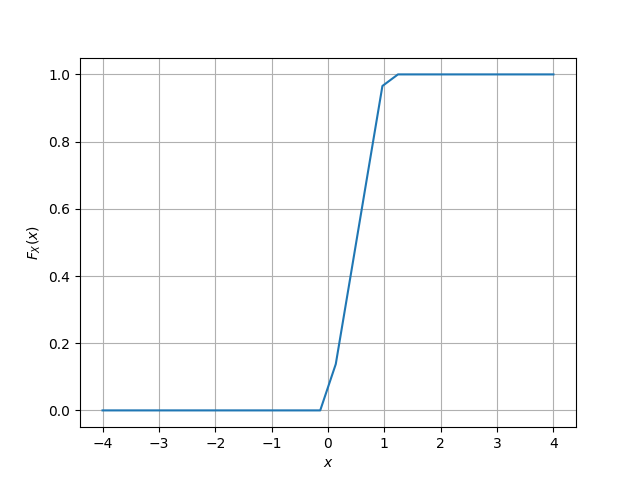
\includegraphics[width=\textheight]{./figures/CDF_uni.png}}
		\label{fig1}
	\end{figure}	
\end{frame}

\section{(1.5)}
\begin{frame}{Solution (1.5)}

    Since 
    \begin{align}
        dF_U(x) = p_U(x) dx
    \end{align}
    we have:
    \begin{align}
        \label{eq2}
        E[U^k] = \int_{-\infty}^{\infty}x^k p_U(x) dx
    \end{align}
    Also,
    \begin{align}
        \label{eq3}
         p_U(x) = 
        \begin{cases}
            0, & x \in (-\infty,0) \\
            1, & x \in (0,1) \\
            0, & x \in (1, \infty)
        \end{cases}
    \end{align}
    \end{frame}
    
    \begin{frame}{Solution (1.5) }
    Therefore, from Equations \ref{eq2} and \ref{eq3}, we have:
    
    \begin{align}
        E[U^2] &=  \int_{-\infty}^{\infty}x^2 p_U(x) dx \\
        &= \int_0 ^1 x^2 dx \\
        &= \frac{1}{3}
    \end{align}
    
    Similarly, 
    \begin{align}
        E[U^2] &=  \int_{-\infty}^{\infty}x p_U(x) dx \\
        &= \int_0 ^1 x dx \\
        &= \frac{1}{2}
    \end{align}
    \end{frame}
    
    \begin{frame}{Solution (1.5)}
    Therefore, the mean is $\frac{1}{2}$, and the variance equals:
    \begin{align}
        E[U^2] - E[U]^2 &= \frac{1}{3} - \brak{\frac{1}{2}}^2 \\
        &= \frac{1}{12}
    \end{align}
    
    
    \end{frame}
    
\section{(2.2/2.3)}
\begin{frame}{Solution (2.2/2.3)}
    We have:
	\begin{align}
		p_X(x) = \frac{1}{\sqrt{2\pi}}\exp{\left(\frac{-x^2}{2}\right)} 
	\end{align}
    Therefore,
    \begin{align}
		F_X(x) &= \int_{-\infty}^{x} \frac{1}{\sqrt{2\pi}}\exp{\left(\frac{-x^2}{2}\right)} \,dx \\
        &= \frac{\text{erf}\left(\frac{x}{\sqrt{2}}\right)+1}{2}
	\end{align}
    where,
    \begin{align}
        \text{erf}(x) = \frac{2}{\sqrt{\pi}} \int _0 ^x e^{-t^2} \,dt 
    \end{align}
\end{frame}

\begin{frame}{Figure (2.2)}
    The empirical and theoretical PDFs are plotted below
	\begin{figure}
		\centerline{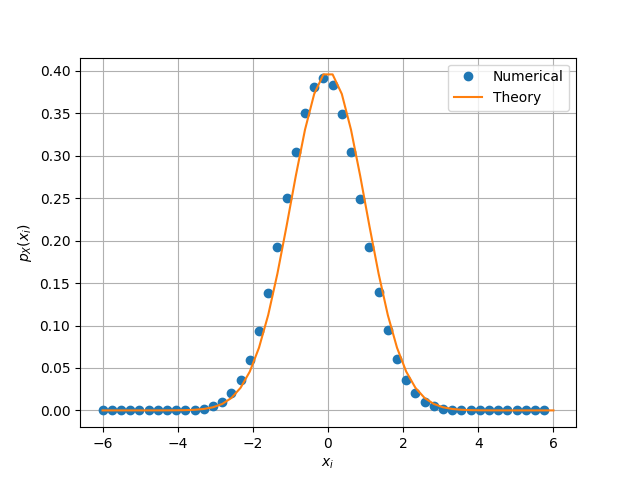
\includegraphics[width=\textheight]{./figures/PDF_gau.png}}
		\label{fig2}
	\end{figure}	
\end{frame}

\begin{frame}{Figure (2.3)}
    The empirical and theoretical CDFs are plotted below
	\begin{figure}
		\centerline{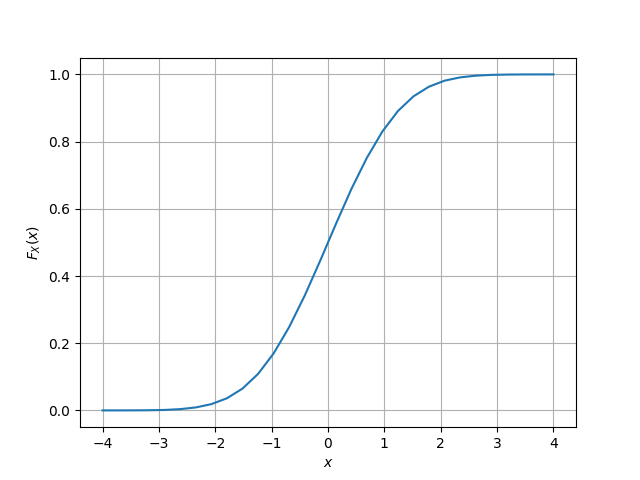
\includegraphics[width=\textheight]{./figures/CDF_gau.png}}
		\label{fig3}
	\end{figure}	
\end{frame}

\section{(2.5)}
\begin{frame}{Solution (2.5)}
    We have:
    
    \begin{align}
        E[X] &=  \int_{-\infty}^{\infty} \frac{x}{\sqrt{2\pi}}\exp{\left(-\frac{x^2}{2}\right)} \\
        &= -\frac{1}{\sqrt{2\pi}}\exp\brak{-\frac{x^2}{2}} \Bigg{|}_{-\infty}^{\infty} \\
        &= 0 
    \end{align}
    
    \end{frame}
    
    \begin{frame}{Solution (2.5)}
    Also,
    
    \begin{align}
        E[X^2] &=  \int_{-\infty}^{\infty} \frac{x^2}{\sqrt{2\pi}}\exp{\left(-\frac{x^2}{2}\right)} \\
        &= -\frac{x}{\sqrt{2\pi}}\exp\brak{-\frac{x^2}{2}} \Bigg{|}_{-\infty}^{\infty} + \int_{-\infty}^{\infty} \frac{1}{\sqrt{2\pi}}\exp\brak{-\frac{x^2}{2}}   \\
        &= 0 + \frac{1}{\sqrt{2\pi}} \times \sqrt{2\pi} \\
        &= 1
    \end{align}
    
    Hence, 
    
    \begin{align}
        \text{var}(X) &= E[X^2] - E[X]^2 \\ 
        &= 1 
    \end{align}

\end{frame}

\section{(3.2)}
\begin{frame}{Solution (3.2)}
    We have:
    
    \begin{align}
    F_V(x) &= \pr{V \leq x} \\
    &= \pr{-2\ln(1-U) \leq x} \\
    &= \pr{1-U \geq	\exp{\left(-\frac{x}{2}\right)}} \\
    &= \pr{U \leq 1 - \exp{\left(-\frac{x}{2}\right)}} \\
    &= F_U\left(1 - \exp{\left(-\frac{x}{2}\right)}\right) 
    \end{align}
    
    \end{frame}

\begin{frame}{Solution (3.2)}
    Therefore,
    \begin{align}
       F_V(x) =
        \begin{cases}
            0, & 1 - \exp{\left(-\frac{x}{2}\right)} \in (-\infty,0) \\
            1 - \exp{\left(-\frac{x}{2}\right)}, & 1 - \exp{\left(-\frac{x}{2}\right)} \in (0,1) \\
            1, & 1 - \exp{\left(-\frac{x}{2}\right)} \in (1, \infty)
        \end{cases}
    \end{align}
    
    From this we get:
    
    \begin{align}
       F_V(x) =
        \begin{cases}
            0, & x \in (-\infty,0) \\
            1 - \exp{\left(-\frac{x}{2}\right)}, & x \in (0,\infty) 
        \end{cases}
    \end{align}
\end{frame}

\begin{frame}{Figure (3.2)}
    The empirical and theoretical CDFs are plotted below
	\begin{figure}
		\centerline{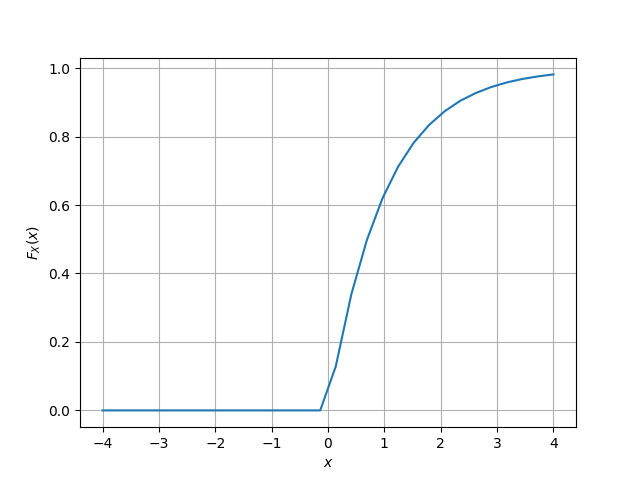
\includegraphics[width=\textheight]{./figures/CDF_log.png}}
		\label{fig4}
	\end{figure}	
\end{frame}


\end{document}